%%%VBS Theory
%\section{Vector Boson Scattering}
\label{section:Vector_Boson_Scattering}

When the scalar field \( \phi \) is expanded around its ground state value, the kinetic term in $\mathcal{L}_\text{Higgs}$ becomes

\begin{equation}
|D_\mu \phi|^2 = \frac{1}{2} (\partial_\mu \phi_0)^2 + \frac{1}{2} (\partial_\mu \phi_2)^2 
+ g^2 \phi_0^2 A_\mu A^\mu + \sqrt{2} g \phi_0 A_\mu \partial^\mu \phi_2 + \ldots,
\end{equation}
where the mass term for \( A_\mu \) is \( g^2 \phi_0^2 A_\mu A^\mu \). The term \( \sqrt{2} g \phi_0 A_\mu \partial^\mu \phi_2 \) provides an extra degree of freedom for \( A_\mu \). The directly coupling \( A_\mu \) to \( \phi_2 \) allows \( \phi_2 \) to serve as an additional degree of freedom for the gauge boson \( A_\mu \), enabling it to acquire the necessary longitudinal polarization to be a massive particle.

A vector boson is a boson with spin-1. By definition, the gauge bosons mentioned above are vector bosons, which introduces Vector Boson Scattering (VBS) into the discussion. 
The SM VBS process involves a quartic gauge coupling (QGC) vertex, as shown in Figure~\ref{fig:qgc_vertex}, which depicts the self-coupling among four electroweak gauge bosons.
The discovery of a Higgs boson in LHC~\cite{20121, 201230} motivates further study of the mechanism of EWSB by probing the VBS processes.
Given that new physics in the electroweak sector is likely to involve QGCs,
the measurements of VBS at high energy are crucial tests of the SM and will determine whether the Higgs is entirely responsible for EWSB.

\begin{figure}[tbp]
\centering
\subfloat[]{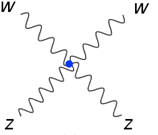
\includegraphics[width=0.27\textwidth]{figures/theory/qgc_1.png}}
\hfill
\subfloat[]{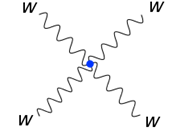
\includegraphics[width=0.3\textwidth]{figures/theory/qgc_2.png}}
\hfill
\subfloat[]{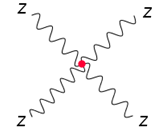
\includegraphics[width=0.27\textwidth]{figures/theory/qgc_3.png}}
\caption{Examples of QGC vertices: (a) and (b) are within the SM; (c) is anomalous, discussed further in Section~\ref{Anomalous_Quartic_Gauge_Couplings}. These and other Feynman diagrams in this thesis are made using the JaxoDraw~\cite{Binosi:2003yf} program.}
\label{fig:qgc_vertex}
\end{figure}

In Figure~\ref{fig:feynmanVBS}, we present examples of VBS diagrams that contribute to the SM signal process in the analysis. 
In the Feynman diagrams presented, a dashed line represents the Higgs boson, a solid line represents quark, and a rippled line represents vector boson.
It's noteworthy that not all VBS diagrams involve quartic gauge couplings. The decays of the bosons are not explicitly shown.

In Figure~\ref{fig:feynmanEWKnonVBS}, we present several non-VBS electroweak diagrams. These include purely-electroweak tree-level diagrams, specifically of order $\mathcal{O}(\alpha_{EW}^6)$, contributing to the final state. Such non-VBS diagrams are expected to be significantly suppressed by the event selection criteria employed in this analysis.

%% feynman diagrams, VBS
%
\begin{figure}[tbp]
\begin{center}
\subfloat[]{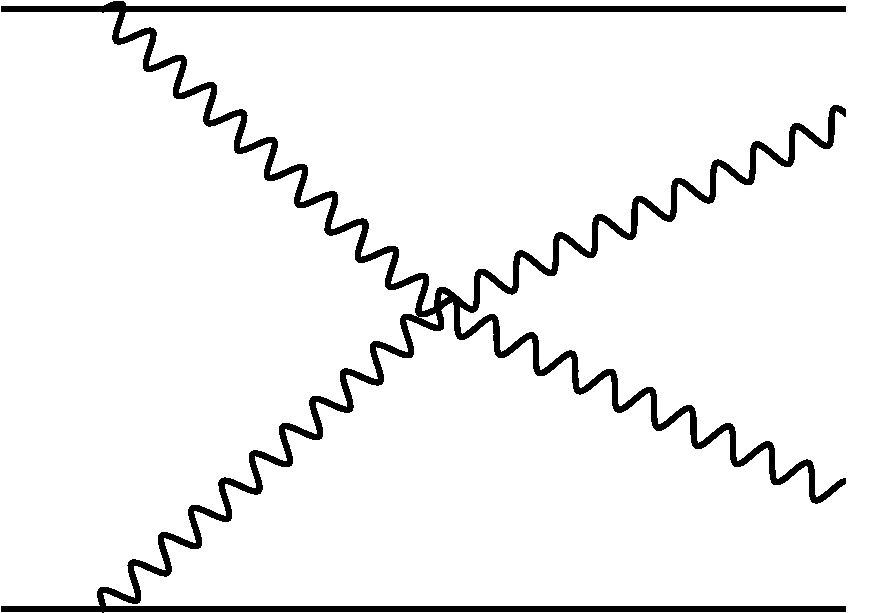
\includegraphics[width=0.3\textwidth]{figures/samples/feynVBS2.pdf}}
\subfloat[]{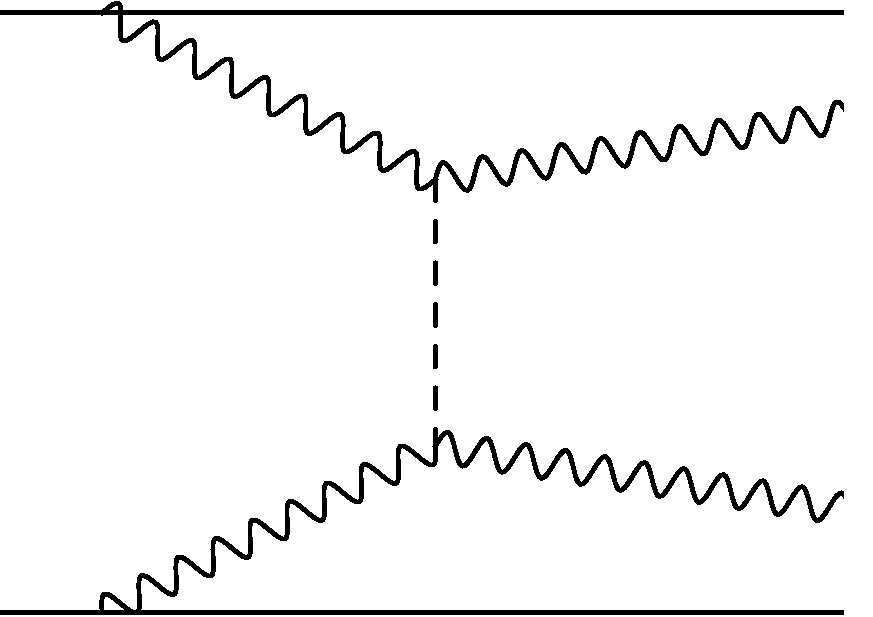
\includegraphics[width=0.3\textwidth]{figures/samples/feynVBS1.pdf}}
\subfloat[]{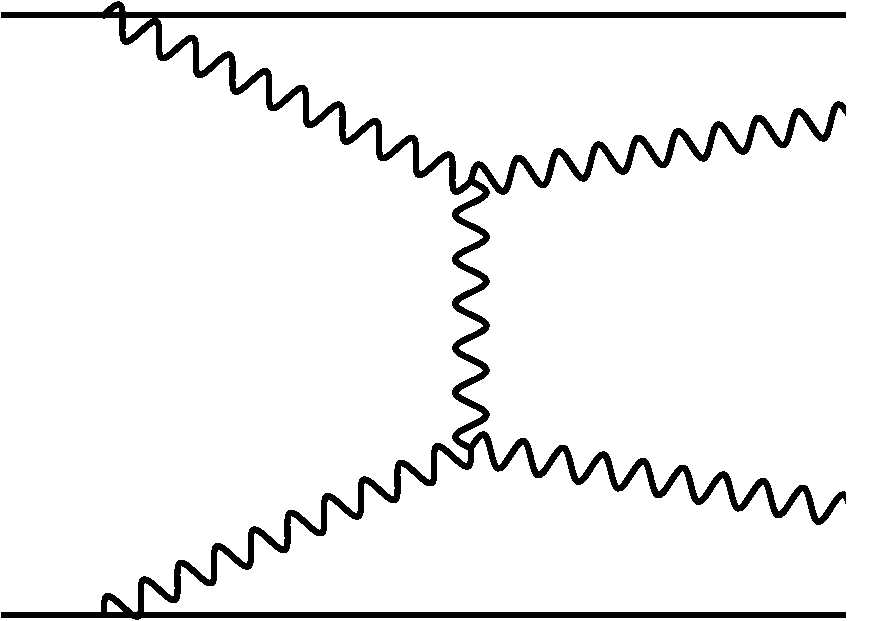
\includegraphics[width=0.3\textwidth]{figures/samples/feynVBS3.pdf}}\\
\subfloat[]{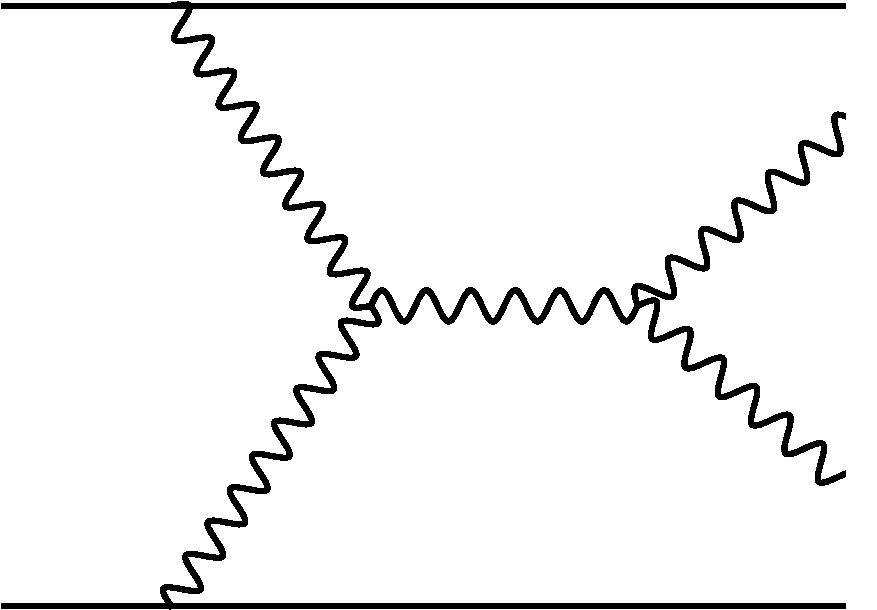
\includegraphics[width=0.3\textwidth]{figures/samples/feynVBS4.pdf}}
\subfloat[]{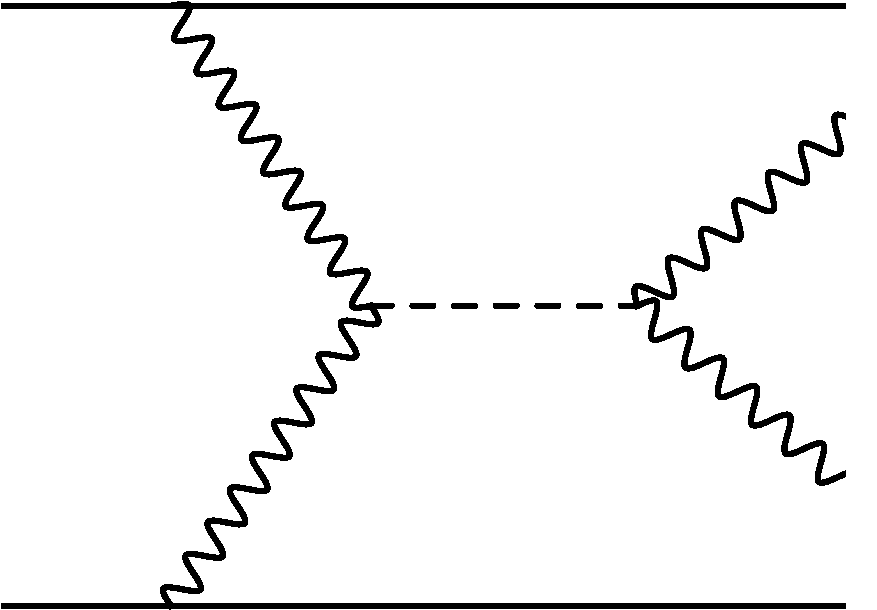
\includegraphics[width=0.3\textwidth]{figures/samples/feynVBS5.pdf}}
\caption{
Examples of VBS diagrams contributing to the signal. Note that not all VBS diagrams contain quartic gauge couplings.
}
\label{fig:feynmanVBS}
\end{center}
\end{figure}


%% feynman diagrams, non-VBS
%
\begin{figure}[tbp]
\begin{center}
\subfloat[]{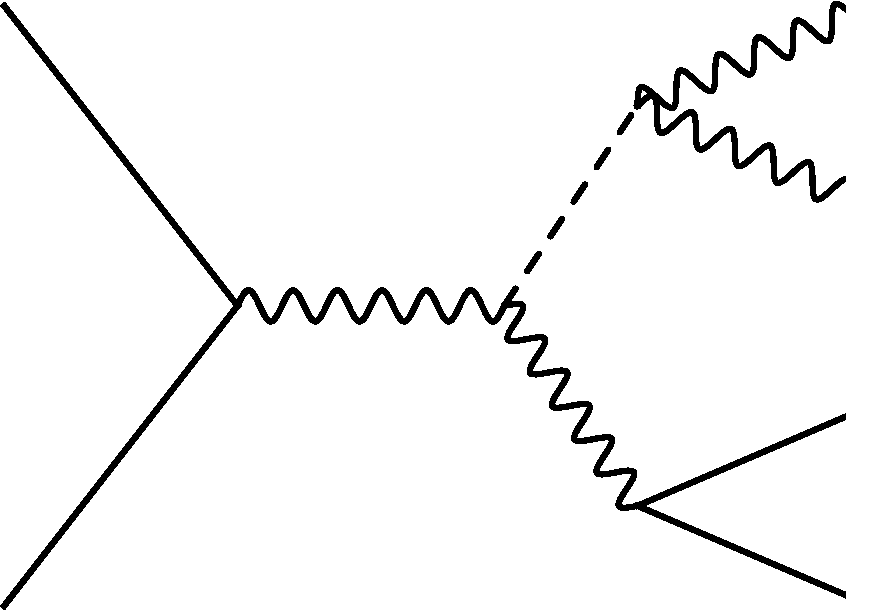
\includegraphics[width=0.3\textwidth]{figures/samples/feynEWKnonVBS3.pdf}}
\subfloat[\label{subfig:feynEWKnonVBSb}]{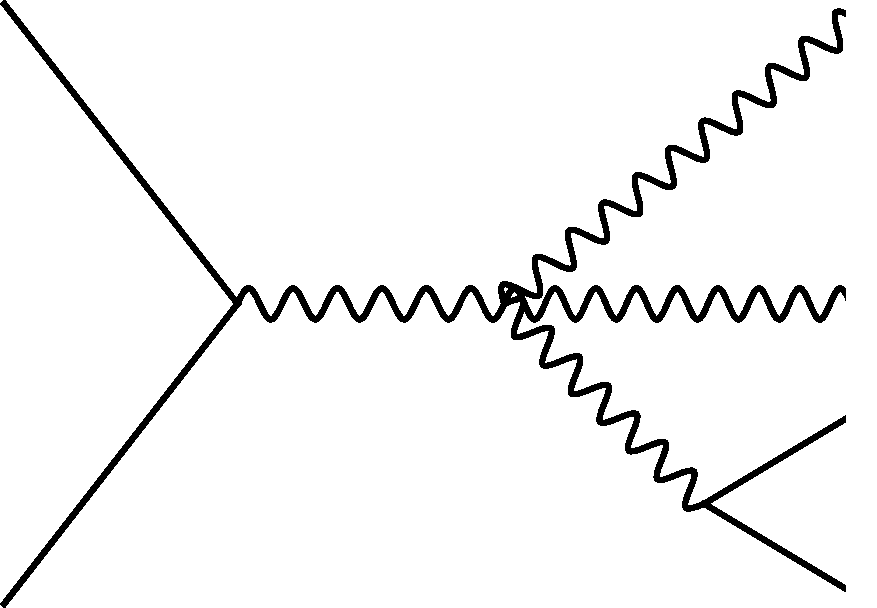
\includegraphics[width=0.3\textwidth]{figures/samples/feynEWKnonVBS4.pdf}}
\subfloat[]{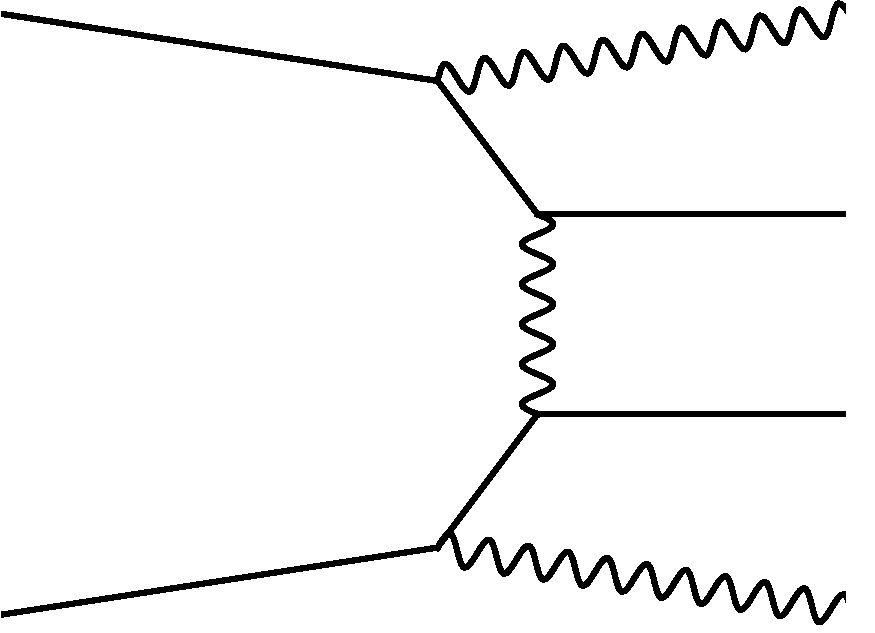
\includegraphics[width=0.3\textwidth]{figures/samples/feynEWKnonVBS5.pdf}}\\
\subfloat[]{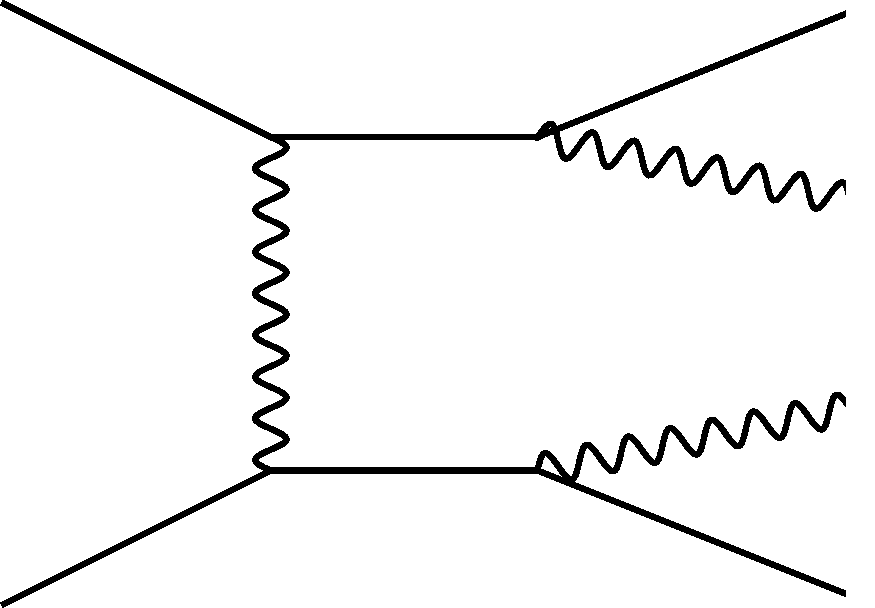
\includegraphics[width=0.3\textwidth]{figures/samples/feynEWKnonVBS6.pdf}}
\subfloat[]{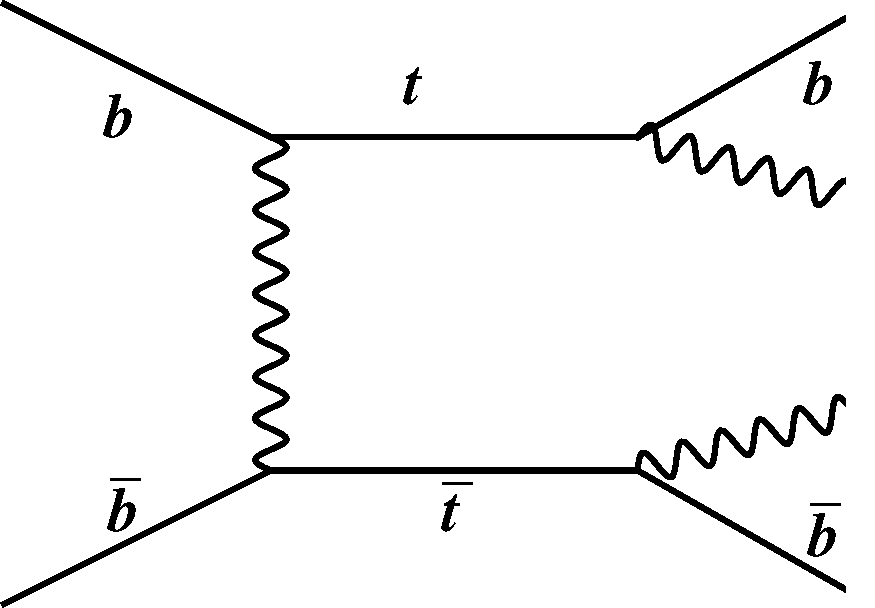
\includegraphics[width=0.3\textwidth]{figures/samples/feynEWKnonVBS1.pdf}}
\subfloat[]{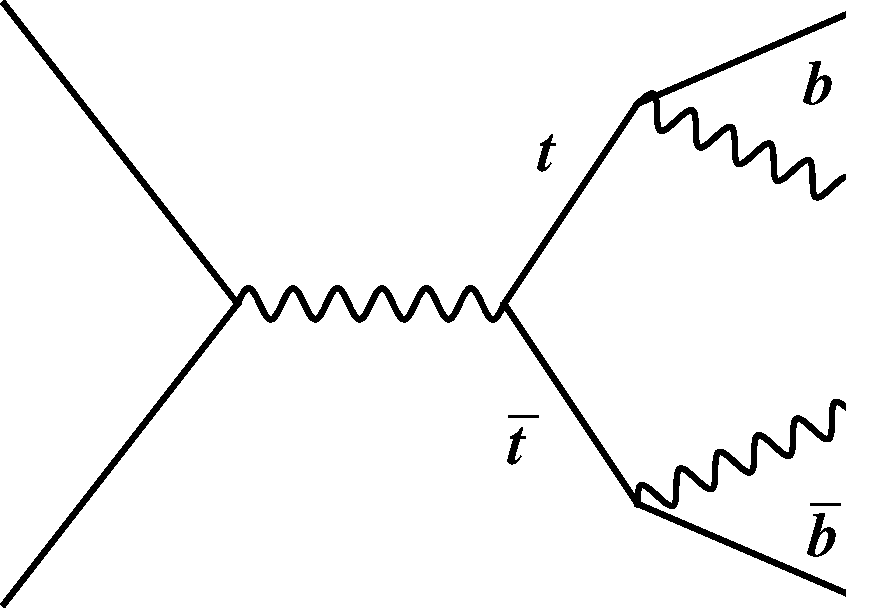
\includegraphics[width=0.3\textwidth]{figures/samples/feynEWKnonVBS2.pdf}}\\
\subfloat[]{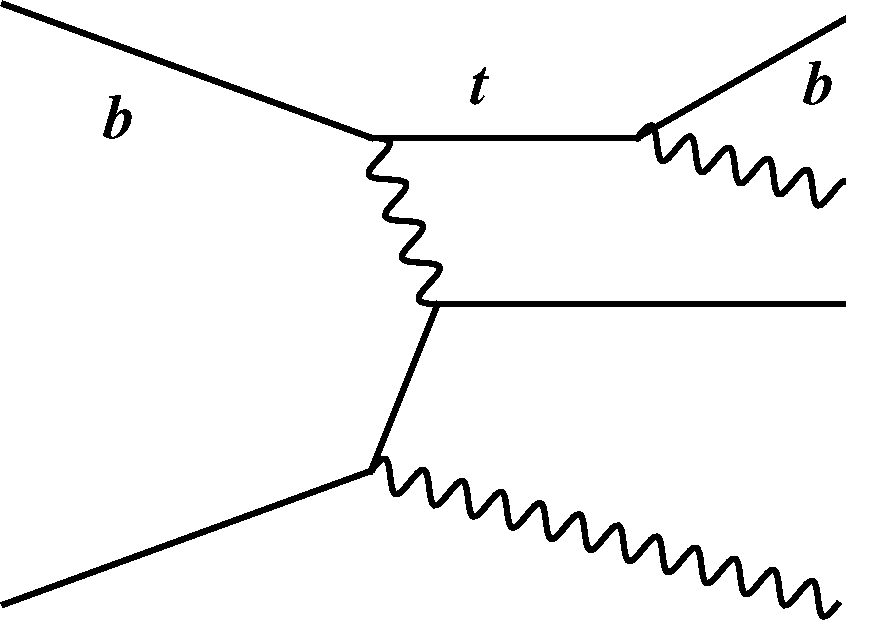
\includegraphics[width=0.3\textwidth]{figures/samples/feynEWKnonVBS7.pdf}}
\caption{
Examples of non-VBS $\mathcal{O}(\alpha_{EW}^6)$ diagrams contributin to the signal.
}
\label{fig:feynmanEWKnonVBS}
\end{center}
\end{figure}

%semileptonic and 1-lepton
Depending on the decay products of the vector bosons, VBS processes can be categorized into three types: fully leptonic, fully hadronic, and semileptonic. 
The fully leptonic VBS analysis studies final states where both vector bosons decay into leptons. 
Similarly, the fully hadronic analysis targets cases where the decay products are exclusively hadronic.
While studies of fully leptonic final states have been done, the branching ratio from double leptonic decay modes is relatively small. On the other hand, fully hadronic final states have a significantly higher branching ratio but introduce considerable background noise, making them challenging to analyze.
The semileptonic VBS analysis is looking at final states with one hadronic and one leptonic boson, offering a balanced compromise between a higher branching ratio and manageable background levels. As illustrated in Figure~\ref{fig:semi_vbs}, the two ``forward'' jets, $j_{f}$ and $j_{b}$, are high \pt jets that scatter through the coupling of the gauge bosons. These jets, pointing roughly along the beamline direction, serve as signatures of the VBS process. Further details on physics object definitions and VBS selection criteria will be discussed in Chapter~\ref{chap:objects_def} and Section~\ref{subsec:vbs_selection}.

Figure~\ref{fig:semi_vbs} also shows two jets, $j_{c}$, orginating from the hadronically decaying vector boson. 
The boson decaying leptonically can have a few conbinations of decay products. 
By counting the number of oberverable lepton(s), we have three channels in the semileptonic VBS analysis. 
Although neutrinos are technically leptons, within the context of this and similar analyses, ``lepton'' typically refers to those detectable directly by the ATLAS and CMS detectors.
Therefore, the 0-lepton channel corresponds to final states where the vector boson decays into a pair of neutrinos.
The 1-lepton channel involves one observable lepton (e.g., $e$, $\mu$) and a neutrino, while the 2-lepton channel includes final states without neutrinos. Most of the work presented in this thesis applies to all three channels but is primarily discussed from the 1-lepton channel perspective.

\begin{figure}[tbp]
\centering
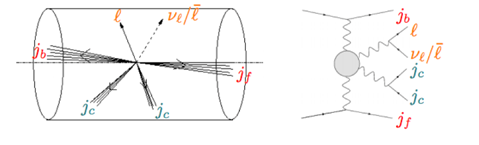
\includegraphics[width=0.75\textwidth]{figures/theory/semi_vbs.png}
\caption{
A schematic representation of a semileptonic VBS process within the detector, accompanied by the corresponding Feynman diagram.
}
\label{fig:semi_vbs}
\end{figure}


%%\begin{figure}[htbp]
%%\centering
%%\begin{subfigure}{.3\textwidth}
%%  \centering
%%\begin{tikzpicture}
%%  \begin{feynman}
%%    \vertex (a);
%%    \vertex [above left=of a] (i1) {\(V_L\)};
%%    \vertex [below left=of a] (i2) {\(V_L\)};
%%    \vertex [above right=of a] (f1) {\(V_L\)};
%%    \vertex [below right=of a] (f2) {\(V_L\)};
%%
%%    \diagram* {
%%      (i1) -- [boson] (a) -- [boson] (f1),
%%      (i2) -- [boson] (a) -- [boson] (f2),
%%    };
%%  \end{feynman}
%%\end{tikzpicture}
%%\end{subfigure}%
%%\begin{subfigure}{.3\textwidth}
%%  \centering
%%\begin{tikzpicture}
%%  \begin{feynman}
%%    \vertex (a);
%%    \vertex [above left=of a] (i1) {\(V_L\)};
%%    \vertex [below left=of a] (i2) {\(V_L\)};
%%    \vertex [right=of a] (b);
%%    \vertex [above right=of b] (f1) {\(V_L\)};
%%    \vertex [below right=of b] (f2) {\(V_L\)};
%%
%%    \diagram* {
%%      (i1) -- [boson] (a) -- [boson] (b)-- [boson] (f1),
%%      (i2) -- [boson] (a),
%%      (f2) -- [boson] (b),
%%    };
%%  \end{feynman}
%%\end{tikzpicture}
%%\end{subfigure}%
%%\begin{subfigure}{.3\textwidth}
%%  \centering
%%\begin{tikzpicture}
%%  \begin{feynman}
%%    \vertex (a);
%%    \vertex [above left=of a] (i1) {\(V_L\)};
%%    \vertex [above right=of a] (i2) {\(V_L\)};
%%    \vertex [below=of a] (b);
%%    \vertex [below left=of b] (f1) {\(V_L\)};
%%    \vertex [below right=of b] (f2) {\(V_L\)};
%%
%%    \diagram* {
%%      (i1) -- [boson] (a) -- [boson] (b)-- [boson] (f1),
%%      (i2) -- [boson] (a),
%%      (f2) -- [boson] (b),
%%    };
%%  \end{feynman}
%%\end{tikzpicture}
%%\end{subfigure}
%%
%%\vspace{2cm}
%%\begin{subfigure}{.3\textwidth}
%%  \centering
%%\begin{tikzpicture}
%%  \begin{feynman}
%%    \vertex (a);
%%    \vertex [above left=of a] (i1) {\(V_L\)};
%%    \vertex [below left=of a] (i2) {\(V_L\)};
%%    \vertex [right=of a] (b);
%%    \vertex [above right=of b] (f1) {\(V_L\)};
%%    \vertex [below right=of b] (f2) {\(V_L\)};
%%
%%    \diagram* {
%%      (i1) -- [boson] (a) -- [scalar, edge label=\(H\)] (b)-- [boson] (f1),
%%      (i2) -- [boson] (a),
%%      (f2) -- [boson] (b),
%%    };
%%  \end{feynman}
%%\end{tikzpicture}
%%\end{subfigure}
%%\begin{subfigure}{.3\textwidth}
%%  \centering
%%\begin{tikzpicture}
%%  \begin{feynman}
%%    \vertex (a);
%%    \vertex [above left=of a] (i1) {\(V_L\)};
%%    \vertex [above right=of a] (i2) {\(V_L\)};
%%    \vertex [below=of a] (b);
%%    \vertex [below left=of b] (f1) {\(V_L\)};
%%    \vertex [below right=of b] (f2) {\(V_L\)};
%%
%%    \diagram* {
%%      (i1) -- [boson] (a) -- [scalar, edge label=\(H\)] (b)-- [boson] (f1),
%%      (i2) -- [boson] (a),
%%      (f2) -- [boson] (b),
%%    };
%%  \end{feynman}
%%\end{tikzpicture}
%%\end{subfigure}
%%\caption{The tree-level Feynman diagrams contributing to VBS process.}
%%\label{fig:feynman_diagrams}
%%\end{figure}


